\documentclass[polish, a4paper, 12pt, oneside]{book}
\linespread{1.3}
\usepackage[a4paper, inner=0cm, outer=0cm, top=2.7cm, right=2.4cm, bottom=2.5cm, left=2.4cm, bindingoffset=1.2cm]{geometry}
\usepackage[utf8]{inputenc}
\usepackage[T1]{fontenc}
\usepackage{lmodern}
\usepackage{microtype}
\usepackage{graphicx}
\usepackage{index}
\usepackage{babel}
\usepackage{csquotes}
\usepackage{xpatch}
\usepackage{enumitem}
\usepackage[]{impnattypo}
\usepackage{polski}
\usepackage{changepage}
\usepackage{indentfirst}
\usepackage{enumitem}
\usepackage{afterpage}
\usepackage{capt-of}
\usepackage[numbers]{natbib}

\bibliographystyle{abbrvnat}
\setcitestyle{authortitle-icmop}
\setlist[itemize,2]{label={$\star$}}

\begin{document}

\begin{titlepage}
	
\includegraphics[height=37.5mm]{agh_nzw_a_pl_3w_wbr_cmyk}\\
	\rule{30mm}{0pt}
	{\large\textsf{Wydział Fizyki i Informatyki Stosowanej}}\\
	\rule{\textwidth}{3pt}\\
	\rule[2ex]
	{\textwidth}{1pt}\\
	\vspace{5ex}
	\begin{center}
	{\bf\LARGE\textsf{Praca inżynierska}}\\
	\vspace{13ex}
	{\bf\Large\textsf{Bartłomiej Mucha}}\\
	\vspace{3ex}
	{\sf \small kierunek studiów:} {\bf\small\textsf{informatyka stosowana}}\\
	\vspace{7ex}
	{\bf\huge\textsf{Migracja serwisów internetowych i integracja usług w środowisku kontenerów Docker}}\\
	\vspace{14ex}
	{\sf \Large Opiekun:} {\bf\Large\textsf{dr inż. Piotr Gronek}}\\
	\vspace{22ex}
	\textsf{\bf\large\textsf{Kraków, styczeń 2020}}
	\end{center}
\end{titlepage}

\vspace*{\fill}
\newpage

\begin{center}
	{\bf\large\textsf{Oświadczenie studenta}}
\end{center}

{\sf Uprzedzony(-a) o odpowiedzialności karnej na podstawie art. 115 ust. 1 i 2 ustawy z dnia 4 lutego 1994 r. o prawie autorskim i prawach pokrewnych (t.j. Dz. U. z 2018 r. poz. 1191 z późn. zm.): ,,Kto przywłaszcza sobie autorstwo albo wprowadza w błąd co do autorstwa całości lub części cudzego utworu albo artystycznego wykonania, podlega grzywnie, karze ograniczenia wolności albo pozbawienia wolności do lat 3. Tej samej karze podlega, kto rozpowszechnia bez podania nazwiska lub pseudonimu twórcy cudzy utwór w wersji oryginalnej albo w postaci opracowania, artystyczne wykonanie albo publicznie zniekształca taki utwór, artystyczne wykonanie, fonogram, wideogram lub nadanie.'', a także uprzedzony(-a) o odpowiedzialności dyscyplinarnej na podstawie art. 307 ust. 1 ustawy z dnia 20 lipca 2018 r. Prawo o szkolnictwie wyższym i nauce (Dz. U. z 2018 r. poz. 1668 z późn. zm.) ,,Student podlega odpowiedzialności dyscyplinarnej za naruszenie przepisów obowiązujących w uczelni oraz za czyn uchybiający godności studenta.'', oświadczam, że niniejszą pracę dyplomową wykonałem(-am) osobiście i samodzielnie i nie korzystałem(-am) ze źródeł innych niż wymienione w pracy.

\bigskip

Jednocześnie Uczelnia informuje, że zgodnie z art. 15a ww. ustawy o prawie autorskim i prawach pokrewnych Uczelni przysługuje pierwszeństwo w opublikowaniu pracy dyplomowej studenta. Jeżeli Uczelnia nie opublikowała pracy dyplomowej w terminie 6 miesięcy od dnia jej obrony, autor może ją opublikować, chyba że praca jest częścią utworu zbiorowego. Ponadto Uczelnia jako podmiot, o którym mowa w art. 7 ust. 1 pkt 1 ustawy z dnia 20 lipca 2018 r. --- Prawo o szkolnictwie wyższym i nauce (Dz. U. z 2018 r. poz. 1668 z późn. zm.), może korzystać bez wynagrodzenia i bez konieczności uzyskania zgody autora z utworu stworzonego przez studenta w wyniku wykonywania obowiązków związanych z odbywaniem studiów, udostępniać utwór ministrowi właściwemu do spraw szkolnictwa wyższego i nauki oraz korzystać z utworów znajdujących się w prowadzonych przez niego bazach danych, w celu sprawdzania z wykorzystaniem systemu antyplagiatowego. Minister właściwy do spraw szkolnictwa wyższego i nauki może korzystać z prac dyplomowych znajdujących się w prowadzonych przez niego bazach danych w zakresie niezbędnym do zapewnienia prawidłowego utrzymania i rozwoju tych baz oraz współpracujących z nimi systemów informatycznych.}

\begin{center}
	\begin{tabular}{lr}
		~~~~~~~~~~~~~~~~~~~~~~~~~~~~~~~~~~~~~~~~~~~~~~~~~~~~~~~~~~~~~~~~~ &
		................................................................. \\
		~ & {\sf (czytelny podpis)}
	\end{tabular}
\end{center}

\tableofcontents{}

\chapter{Wstęp}
Możliwości, jakie oferują maszyny wirtualne są nieocenione we współczesnym świecie. Systemy serwerowe, w skład których mogą wchodzić nawet tysiące powiązanych ze sobą lub indywidualnych serwisów, nie mogą występować albo są zasadniczo trudne do wdrożenia na jednej platformie o określonym systemie opracyjnym, konfiguracji i innych elementach wchodzących w skład szeroko rozumianego środowiska. Maszyny wirtulane są rozwiązaniem tego zagadnienia. Każda maszyna wirtualna może zostać stworzona niezależnie od architektury sprzętowej i oferuje dowolone środowisko, które jednocześnie będzie wyizolowane od środowisk gospodarza (\textit{host}) i innych maszyn wirtualnych (\textit{guest}). Korzyścią płynącą z izolacji środowiska jest chociażby zwiększone bezpieczeństwo systemu, ułatwienie zarządzania serwisami oraz wdrażania nowych wersji aplikacji. Nierzadko używane są stare serwisy, a jednak spełniające swoje zadanie, które wymagają rozwiązań nieaktualnych już wersji elementów środowiskowych, nie wspieranych przez nowsze wersje. Co za tym idzie wdrożenie np. dwóch aplikacji działających w ramach tej samej technologii, ale na różnych wersjach będzie tworzyć konflikt. Problemy tego typu zanikają w kontekście wirtualzacji, albowiem nic nie stoi na przeszkodzie osadzenia każdej pojedynczej aplikcaji na osobnej maszynie. Wirtualizacja posiada jednak szereg wad. Taką wadą jest na przykład to, że każda maszyna wirtualna musi rezerwować określoną i niezmienną w czasie działania ilość zasobów, takich jak pamięć operacyjna (np. \textit{RAM}) i masowa (nieulotna) oraz liczbę wątków procesora i wiele innych. Stawia to przed adminstratorem problem, związany z dobraniem parametramów jakimi taka maszyna ma się cechować. Przydzialnie zbyt małej ilości zasobów sprawi, że serwis będzie niedomagał. Z kolei przydzielnie zbyt dużej ilości zasobów doprowadzi do marnowania się części zasobów, które mogłyby być lepiej wykorzystane. To, jak maszyna wirtualna zużywa zasoby, takie jak pamięć operacyjna, nie jest kontrolowane. Zarezerwowany zasób jest statyczny i nie jest zwalniany w przypadku braku użycia. Rozwiązaniem tego problemu jest zmiana podejścia do koncepcji wirtualzacji, a mianowicie konteneryzacja serwisów. Platformy takie jakie \textit{Docker}\cite{docker} czy \textit{LXC}\cite{lxc} pozwalają tworzyć niewymagające udziału hipernadzorcy wyizolowane środowiska o dynamicznie przydzielanych zasobach, tak zwane kontenery. Kontenery zarządzane przez platformę Docker współdzielą jądro systemowe z gospodarzem i innymi kontenerami, a w ramach osadzenia aplikacji wystarczy dostarczyć zbudowaną aplikację oraz wymagane do poprawnego jej działania składniki systemowe. W ten sposób można zaoszczędzić na użyciu pamięci twardej względem tej samej aplkacji wdrożnej na maszynie wirtualnej. 

\section{Cel pracy}
Celem pracy jest przeniesienie aplikacji z maszyn wirtualnych na kontenery oraz opracowanie tej metodologii. W konsekwencji zostaną stworzone skalowalne środowiska usług internetowych, działające w oparciu o technologię kontenerów Docker na platformie Linux w systemie wirtualizacji \textit{VMware ESX}\cite{vmwareesx} oraz porównanie i ocena korzyści wynikających z tych działań. Modelem przykładowym jest system aplikacji działających w technologii \textit{Php}\cite{php} i \textit{Java}\cite{java} z framework'iem \textit{Spring Boot}\cite{springboot} oraz baza danych \textit{PostgreSQL}\cite{postgresql} na trzech osobnych kontenerach Docker. Kontenery będą osadzone na zainstalowanej w systemie wirtulazacji ESX maszynie wirtualnej z system operacyjnym \textit{Debian 10}\cite{debian10}. Finalnie wdrożone zostaną realne serwisy w wydziałowej sieci komputerowej.
%\begin{center}
%	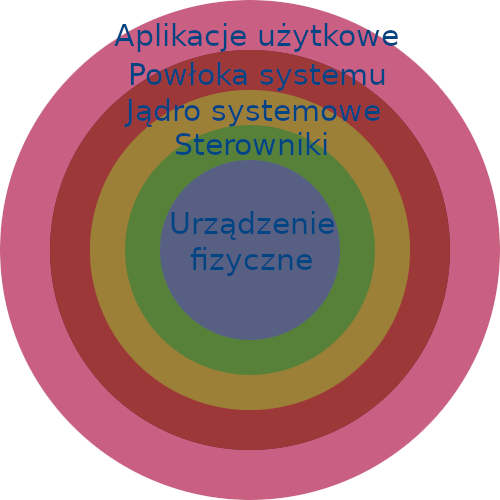
\includegraphics[height=100mm]{schemat_os.png}
%	\captionof{figure}{Schmat warstw systemu operacyjnego}
%\end{center}

Plan pracy jest następujący. W części teortycznej zostaną omówione mechanizmy stojące za działaniem maszyn wirtualnych i kontenerów na platformie Docker oraz ich porównanie. Natępnie omówiony zostanie schemat wdrożenia aplikacji. Część praktyczna będzie zawierać szczegółowy opis przygotowania środowiska oraz wdrożenia aplikacji zarówno przykładowych. 

\section{Założenia projektu}
Celem projektowej części pracy jest opracowanie skalowalnego środowiska usług internetowych, działającego w oparciu o technologię kontenerów Docker na platformie \textit{Linux} w systemie wirtualizacji \textit{VMware ESX}\cite{vmwareesx}. Usługi realizowane przez system mają obejmować obsługę: - internetowych serwisów aplikacyjnych działających w technologiach odpowiednio: \textit{Php}\cite{php}, \textit{Apache Tomcat}\cite{apachetomcat}, \textit{Python}\cite{python} \textit{Django}\cite{django}, witryn \textit{CMS WordPress}\cite{wordpress}, serwerów relacyjnych baz danych \textit{MySQL}\cite{mysql}, \textit{PostgreSQL}\cite{postgresql}. Elementem pracy będzie także migracja istniejących serwisów internetowych do ich odpowiadających im instancji wyżej wymienionych kontenerów \textit{Docker}\cite{docker} oraz ocena uzyskanych korzyści pod kątem konsumowanych zasobów sprzętowych i wydajności działania. 

\chapter{Podstawa Teoretyczna}
\section{Wirtualizacja}
Szeroko rozumiane urządzenie zwane komputerem składa się z dwóch kategorii komponentów: urządzeń fizycznych i oprogramowania. W skład urządzeń fizycznych wchodzą między innymi płyta główna, centralna jednostka przetwarzająca i urządzenia wejścia/wyjścia. Oprogramowanie składa się z warstw, najniżej, najbliżej sprzętu znajduje się oprogramownie do zarządzania i komunikacji z urządzaniami, w wyższych warstwach znajdziemy aplikacje użytkowe. Zadaniem systemu operacyjnego jest zarządzanie zarówno zasobami sprzętowymi jak i oprogramowaniem. Stanowi on interfejs pomiędzy maszyną a użytkownikem, umożliwiając tym samym stosowanie komputerów do celów osobistych znanych nam z życia codziennego i profesjonalnych na linii człowiek - maszyna, ale i maszyna - maszyna. Ideą systemu operacyjnego jest istnienie środowiska, które dynamicznie będzie tłumaczyć zlecenia użytkownika na język maszynowy, następnie zlecać sprzętowi ich wykonanie i w drugą stronę informować użytkownia o rezultatach pracy maszyny oraz jej zapotrzebowaniu na dane, zachowując jednocześnie optymalne działanie pracy całego systemu i zawartych w nim urządzeń.
   
\begin{center}
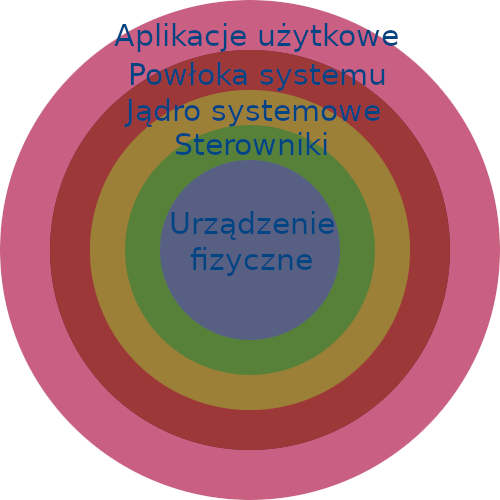
\includegraphics[height=100mm]{schemat_os.png}
\captionof{figure}{Schmat warstw systemu operacyjnego}
\end{center}

Na rysunku 2.1 przedstawiony jest schemat budowy systemu operacyjnego. W skład samego systemu operacyjnego wchodzą sterowniki, jądro i powłoki systemowe. System operacyjny jest również podzielony na przestrzenie jądra i użytkownika. Wirtualizacja zatem jest symulacją warstwy fizycznej komputera, na której można zainstalować i używać dowolny system operacyjny. Zasymulować można różnego rodzaju architektury i parametry sprzętowe, zalecane jest jednak by wirtualna platforma sprzętowa nie przekraczała możliwości rzeczywistego sprzętu. Wirtualizacji można dokonać na kilku poziomach. 
\subsection {Poziom architektury zestawu instrukcji (\textit{ISA})}
Tak zwana pełna wirtualizacja. Wszytkie instrukcje procesorowe systemu gościa są interpretowane przez emulator, a następnie mapowane na rzeczywisty sprzęt fizyczny gospodarza. Dalej instrukcje są wykonywane i zwracane do emulatora, który przekazuje je do gościa. Z racji długiej drogi, jaką musi pokonać pojendyczna instrukcja to rozwiązanie należy do najwolniejszych. Tę metodę stosuje się, gdy architektury sprzętowe gościa i gospodarza są zbyt różne, aby dało się je zmapować lub jest to nieopłacalnie trudne. Rozwiąnie to stosuje się na przykład do emulacji środowisk smartfonów, konsol do gier i mikrokontrolerów.
\subsection {Poziom warstwy abstrakcji sprzętowej (\textit{HAL})}
Inaczej nazywany poziomem sprzętowego wspomagania. Ta metoda wirtulizacji polega na mapowaniu rzeczywistych zasobów sprzętowych na wirtualne zasoby. Zatem wszystkie instrukcje nieuprzywilejowane są wykonywane bezpośrednio na sprzęcie gospodarza. Instrukcje uprzywilejowane, czyli takie które może wykonać tylko gospodarz są przekazywane do hipernadzorcy i ten je wykonuje. Rozwiąznie to jest zasadniczo szybsze od wirtualizacji zestawu instrukcji. Z tej metody korzystają narzędzia do wirtualizacji takie jak \textit{VMware Workstation}\cite{vmwareworkstation}, \textit{Oracle VirtualBox}\cite{virtualbox} i wiele innych.
\subsection {Poziom systemu operacyjnego}
Wirtualizacja na poziomie systemu opercyjnego pozwala na działanie kilku odrębnych odizolowanych od siebie systemów operacyjnych, a dokładnie przestrzeni użytkownia korzystających z jednego jądra systemowego. Zatem nie dochodzi do duplikacji całych systemów operacyjnych, a co za tym idzie nie jest wymagana praca hipernadzorcy. Rozwiązanie takie jest nazywane konteneryzacją i jest stosowane na takich platformach jak Docker, \textit{CoreOS}\cite{coreos}, \textit{LXC}\cite{lxc} i \textit{Oracle Solaris Containers}\cite{solaris}. Wadą tej metody jest przymus używania tylko takich systemów operacyjnych, które mogą współdzielić jądro z systemem gospodarza. Nic jednak nie stoi na przeszkodzie, aby umieścić kontenery na maszynie wirtualnej postawionej na poziomie wspierania sprzętowego, jednak spowolni to szybkość tych kontenerów do szybkości samej maszyny wirtualnej. 
\subsection {Poziom bibliotek lub języków programownia}
Poziom ten jest stosowany w ramach technologii \textit{JIT} (\textit{just in time}). Niektóre środowiska programistyczne pozwalają na kompilację kodu źródłowego do postaci kodu pośredniego, który nie ma bezpośredniego przełożenia na kod maszynowy. Program jest wykonywany na maszynie wirtualnej, która kompiluje kod pośredni do kodu maszynowego, a może to zrobić na poczatku wywołania programu lub pierwszego wywołania konkretnej części kodu. Z tej technologii korzysta \textit{Java}\cite{java}, \textit{.Net}\cite{dotnet}, \textit{Python}\cite{python} i wiele innych języków programowania. 
\subsection {Poziom aplikacji}
Wirtualizowane są tylko aplikacje, co oznacza, że nie wykorzystują one bezpośrednio dostarczanego przez system operacyjny środowiska wykonawczego, a używją dostarczonego przez inną aplikację takie środowisko na jakie zostały zbudowane. Przykłądem platformy umożliwijącej wirtualizacje aplikacji jest \textit{Wine}\cite{wine}, która umożliwia działanie aplikacji przystowanych do pracy w systemie \textit{Microsoft Windows}\cite{windows} na systemie operacyjnym typu Linux.
 
\section{Hipernadzorca}
Komponentem systemu komputerowego umożliwiającym dokonanie wirtualizacji na poziomie wsparcia sprzętowego jest hipernadzorca (\textit{hypervisor}). Rozróżnanie są dwa typy hipernadzorców:

\subsection {Hipernadzorca typu pierwszego} 
Jest to tak zwany hipernadzorca natywny (\textit{bare metal}) osadzony bezpośrednio na sprzęcie, nie wymaga on zainstalowanego systemu operacyjnego gospodarza. Pozwala on osadzać maszyny wirtualne nad sobą, co znacząco upraszcza schemat abstrakcji architektury całego systemu. Przykładami tego typu hipernadzorców są \textit{Microsoft Hyper-V}\cite{hyperv} i \textit{VMware ESXi}\cite{vmwareesx}.
%\begin{center}
%	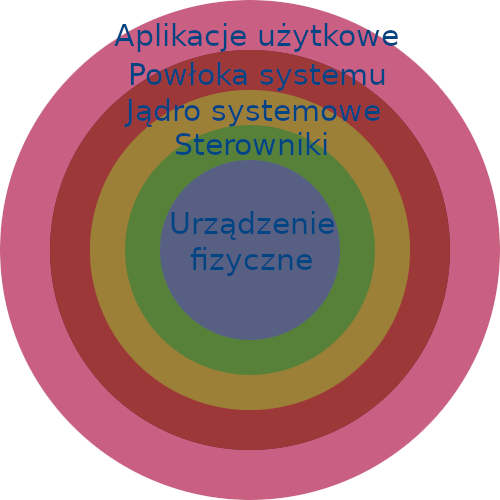
\includegraphics[height=100mm]{schemat_os.png}
%	\captionof{figure}{Schmat warstw systemu operacyjnego}
%\end{center}

\subsection {Hipernadzorca typu drugiego} 
Hipernadzorca hostowany jest osadzony w systemie operacyjnym gospodarza jako aplikacja. Takimi aplikacjami są przykładowo \cite{VMware Workstation}, \textit{VMware Player}\cite{vmwareplayer}, \textit{Oracle VirtualBox}\cite{virtualbox} i \textit{QEMU}\cite{qemu}.
%\begin{center}
%	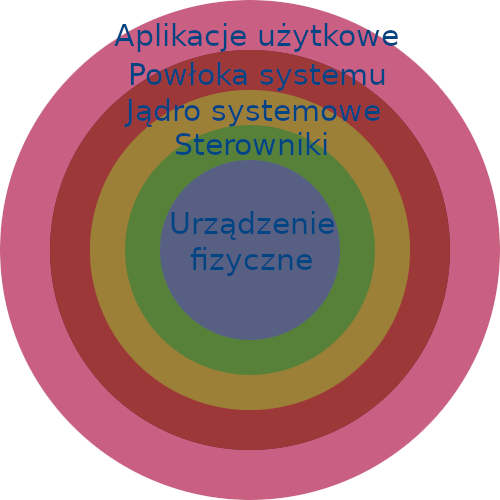
\includegraphics[height=100mm]{schemat_os.png}
%	\captionof{figure}{Schmat warstw systemu operacyjnego}
%\end{center}

\section{Konteneryzacja}
Konteneryzacja jako wirtualizacja na poziomie systemu opercyjnego, z racji wspóldziełenia przez kontenery jądra systemu gospodarza, powinna cechować się większą wydajnością od wirtulizacji na poziomie \textit{ISA} lub \textit{HAL}. O ile nie zastąpi ona klasycznych maszyn wirtualnych pod względem możliowści uruchamiania różnorodnych systemów operacyjnych, o tyle najmocniejszą stroną konteneryzacji jest dużo niższe zapotrzebowanie na pamięć nieulotną, co za tym idzie przenaszalność oraz szybkość zarówno działania jak i startowania. Współdzielenie jądra systemowego oraz dostępu do fizycznej warstwy komputera niesie ze sobą pewne ryzyko jakim jest drastyczny spadek wydajności. Wszystkie kontenery konkurują ze sobą o zasoby sprzętowe, ale również o zasoby jądra, które nie jest odizolowne między nimi. Zespół Sysdig napotkał na problem degradacji szybkości działania środowiska wewnątrz kontenerów. Z artykułu autorstwa Gianluca Borello\cite{sd17} wynika, że jeden kontener spowalniał inny, poprzez wielkrotne wyszukiwania plików o zadanych ścieżkach dostępu. Proces rozwikłania scieżek dostępu jet procesem nietrywilanym i czasochłonnym, jądro \textit{Linuxa} zapisuje w związku z tym dane jakie uzyskał w tablicy haszowanej, również próby nieudane, by w pszyszłości nie powtarzać całego procesu. Ma to na celu szybsze rozwikłania ścieżek. Jeżeli jednak dojdzie do nadmierngo rozrostu tablicy to efekt staje się odwrotny do zamierzonego i jądro działa wolniej, tym samym spowalniając uruchomione w każdej przestrzeni użytkownika apliakcje. Jądro systemu jest bardzo skomplikowanym oprogramowaniem i jak każde oprogramowanie może w pewnych warunkach nie działać optymalnie, jak w wymienionym przypadku i innych tworząc wąskie gardło pomiędzy warstwami użytkownika i warstwą fizyczną.

%\begin{center}
%	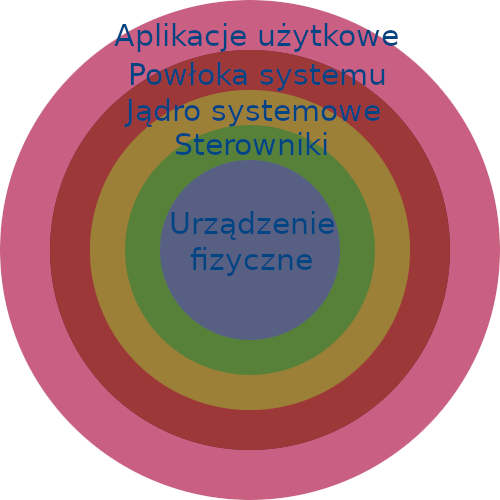
\includegraphics[height=100mm]{schemat_os.png}
%	\captionof{figure}{Schmat warstw systemu operacyjnego}
%\end{center}

\chapter{Założenia projektowe}
\section{Architektura wejściowa serwisów}
\subsection{Platforma systemu serwerowego}
Na wydziałowym serwerze zainstalowny jest hipernadzorca typu pierwszego, dokładnie \textit{VMware ESX 6.5}\cite{vmwareesx}, osadzony bezpośrednio nad warstwą fizyczną klastra komputerowego. Na serwerze wdrożonych jest szereg aplikacji działających na odrębnych maszynach wirtulanych. 

\subsection {Wizualizaja platformy wejściowej} Na rysunku x.x znajduje się schemat wejściowej architektury systemu serwerowego, który w ramach tej pracy ma zostać przekształcony.
%\begin{center}
%	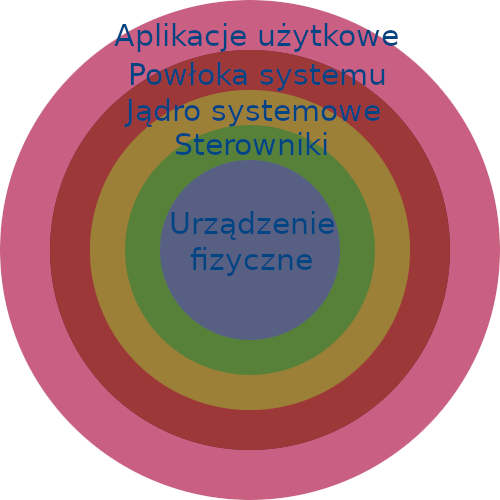
\includegraphics[height=100mm]{schemat_os.png}
%	\captionof{figure}{Schmat warstw systemu operacyjnego}
%\end{center}

\section{Architektura docelowa serwisów}
Koncepcja architektury docelowej polega na zlikwidowaniu pewnej ilości maszyn wirtulanych i przeniesieniu serwisów w nich zawartych do kontenerów znajdujących się w jednej maszynie wirtualnej. Oczywistą korzyścią z tej akcji jest zaoszczędzenie pewnej, być może nawet dużej ilości  pamięci twardej. Nie jest jednak oczywiste, do jakiej zmiany dojdzie w kwestii wydajności. O ile pierwotny układ składa się z jednego poziomu wirtualizacji, tak ten układ będzie się składał z dwóch: wirtualizacji wspomaganej sprzętowo oraz na poziomie systemu operacyjnego.
%\begin{center}
%	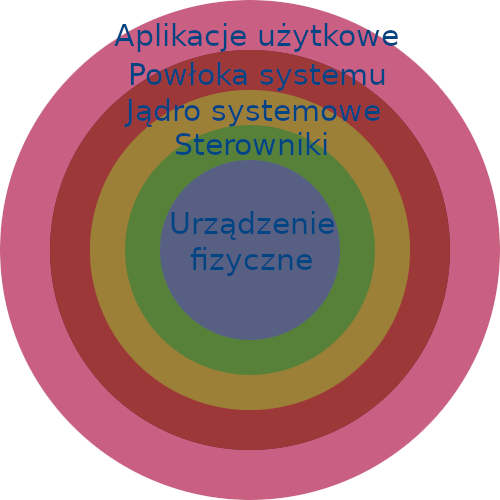
\includegraphics[height=100mm]{schemat_os.png}
%	\captionof{figure}{Schmat warstw systemu operacyjnego}
%\end{center}

\chapter{Opis przykładowych aplikacji}
\section{Opis}
Przykładowe aplikacje to najprostsze aplikcje o identycznych wymaganiach jak aplikacje pochodzące z wydziałowego serwera. Aplikacja Java Spring Boot jest naprostszym serwisem http wyświetlający prostą zawartość w przeglądarce internetowej. Serwis Apache-Php również jest serwisem http, który udostępnia przez przeglądarkę interfejs \textit{CRUD} do trzeciego serwisu, który dostarcza bazę danych PostgreSQL.  
\section{Środowisko projektowe i wymagania aplikacji}
\subsubsection{Środowisko projektowe:}
\begin{itemize}[noitemsep]
    \item Narzędzie do wirtualizcji \textit{VMware Workstation Player 15.5}\cite{vmwareplayer}
    \item System operacyjny \textit{Debian 10.2}\cite{debian10}
    \item platforma \textit{Docker 19.03.5}\cite{docker}
    \item narzędzie do zarządzania kontenerami \textit{Docker-compose 1.25.0}\cite{dockercompose}
\end{itemize}

\subsubsection{Wymagania Aplikacji:}
\begin{itemize}[noitemsep]
    \item Aplikacja \textit{Java Spring Boot}
    \begin{itemize}[noitemsep]
    	\item \textit{Java 8}\cite{java} lub nowsza
    \end{itemize}
    \item Aplikacja \textit{Php}
	\begin{itemize}[noitemsep]
		\item \textit{Php 5.4}\cite{php} lub nowsze z dodatkiem umożliwiającym połączenie z bazą danych PostgreSQL
		\item \textit{Apache 2}\cite{apache} lub nowszy
		\item Dostęp do istniejącej bazy danych \textit{PostgreSQL}\cite{postgresql}
	\end{itemize}
\end{itemize}

\section{Działanie i powiązania zbioru kontenerów}
\subsubsection{Docker}
Platforma Docker do utworzenia kontenera wymaga dwóch komponentów: zbudowanej aplikacji i jej zasobów w postaci na przykład plików html, skryptów itd. oraz pliku konfiguracyjnego \textit{dockerfile}, na podstawie którego zostanie utworzona przestrzeń użytkownika w kontenerze. Wykorzystanymi komendami \textit{dockerfile} w projekcie są:
\begin{itemize}[noitemsep]
	\item \textit{RUN} wykonuje polecnie powłoki systemu operacyjnego w konenerze podczas jego budowy
	\item \textit{CMD} nadpisuje domyślną instrukcję \textit{command}, która domyślnie uruchamia aplikacje wewnątrz kontenera. Dotyczy to przypadku, w którym kontener pracuje w trybie odłączonym od powłoki systemu gospodarza. Instrukcja \textit{CMD} może zostać wykorzystana raz, każda kolejna nadpisze poprzednią, w konsekwencji wykonana zostanie tylko ostatnia.
	\item \textit{COPY} kopiuje pod podane miejsce w systemie plików gościa wskazane pliki i katalogi z systemu plików gospodarza
	\item \textit{ADD} jest to rozszerzona instrukcja \textit{COPY}, pozwala również na dodanie plików z pod podanego adresu \textit{url} oraz automatycznie rozpakować foldery skompresowane w trakcie kopiowania
	\item \textit{ENTRYPOINT} wykonuje tę samą czynność co \textit{CMD} z tą różnicą, że może być użyta wielokrotnie i każde użycie zostanie wykonane. Instrukcje \textit{ENTRYPOINT} i \textit{CMD} nie kolidują ze sobą
	\item \textit{VOLUME} tworzy obszar w pamięci twardej gospodarza, w którym będzie przechowywana kopia danych wygenerownych przez kontener, np. logi, bazy danych itd.
	\item \textit{FROM} instrukcja, której obecność jest zawsze wymagana do zbudowania obrazu. Musi znajdować się w pierwszej linii pliku docker file. Jej argumentem jest tag obrazu który ma zostać zbudowny. W trakcie budowy obraz jest pobierany z repozytorium.
	\item \textit{ENV} tworzy zmienną środowiskową w goszczonym systemie opercyjnym
	\item \textit{EXPOSE} pokazuje port widoczny dla maszyn zewnętrznych
\end{itemize}
Z racji tego, iż wybranym system opercyjnym gospodarza dla kontenerów jest \textit{Debian 10}\cite{debian10}, \textit{dockerfile} musi zawierać komendy, które zainstalują wymagane do działania aplikacji paczki i biblioteki oraz koniecznie musi korzystać z obrazów systemów z rodziny \textit{Linux}.
\subsubsection{Docker-compose}
W przypadku kiedy w systemie pracuje wiele kontenerów pojawia się problem zarządzania nimi. Uruchamianie każdego kontenera z wiersza poleceń jest żmudnym i podatnym na pomyłki procesem. Zastosowanie skryptu np. w powłoce bash cechowałoby się nie małą nieprzerzystością. Programem służącym do tego celu jest \textit{Docker-compose}. Pozwala on budowanie i uruchamianie wielu kontenerów docker jednocześnie. Tak jak \textit{Docker}\cite{docker}, \textit{Docker-compose}\cite{dockercompose} wymaga pliku konfiguracyjnego, tym razem w notacji \textit{YAML} i o rozszerzeniu \textit{docker-compose.yml}. W tym pliku są zawarte lokacje plików dockerfile i parametry służące do budowy i uruchomienia obrazu oraz konfiguracja sterowników np. sieciowych. 
\subsubsection{Aplikacja Java Spring Boot}
Realizuje prosty zadanie, tworzy serwis internetowy i wyświetla przykłądowy napis oknie przeglądarki.
\subsubsection{Aplikacja Php}
Zadaniem tej aplikacji jest zainicjalizowanie bazy danych i udostępnienie za pośrednictwem strony \textit{www} interfejsu \textit{CRUD} do tej bazy.
\subsubsection{Baza danych PostgreSQL}
Baza danych musi istnieć i być dostępna dla aplikacji \textit{Php}
\section{Zrealizowane pliki dockerfile}

\chapter{Wdrożenie przykładowych oraz rzeczywistych serwisów wydziałowego systemu informatycznego}
\section{Wdrożenie przykładowych aplikacji}
Wdrożenie utowrzonego systemu w ramach tej pracy polega na imporcie maszyny wirtualnej zawierającej gotowe środowisko i aplikacje do środowiska VMware ESX na wydziałowym systemie serwerowym. Po rozwiązaniu kliku pomniejszych problemów z konfiguracją dostarczonej maszyny wirtualnej udało się ostatecznie ją zainstalować i uruchomić. Zbudowne ówcześnie kontenery zostały wzbudzone komendą: \texttt{docker-compose up}. Operacja zakończyła się pełnym sukcesem, serwisy działały poprawnie i były widoczne dla wszystkich urządzeń sieci wydziałowej.

\section{Wdrożenie rzeczywistych serwisów wydziałowego systemu informatycznego}

\chapter{Wnioski}

\chapter{Kod źródłowy}
\section{Repozytorium Git}
\section{Dołączona płyta CD}

%\chapter {Bibliografia}
\bibliography{bibliografia}

\end{document}